\documentclass{article}
\usepackage[T1]{fontenc}
\usepackage{graphicx}
\usepackage{amsmath, amsthm, amssymb}
\usepackage{hyperref}
\usepackage{polski}
\usepackage{array}
\usepackage{float}
\newtheorem{theorem}{Twierdzenie}
\usepackage[a4paper, left=1.5cm, right=3cm, top=2cm, bottom=2cm]{geometry}
\theoremstyle{definition}
\usepackage{enumerate}
\usepackage{listings}
\usepackage{color}
\newtheorem{definition}{Definicja}

\title{Sprawozdanie Lista2}
\author{Paweł Solecki}
\date{\today}
\begin{document}
	\maketitle
	\section{Zadanie 1: Quick\_Sort}
	Quick sort to algorytm sortowania, który dzieli tablicę na dwie części względem wybranego elementu zwanego pivotem, a następnie sortuje każdą z części rekursywnie.
	\begin{lstlisting}[language=C++, tabsize=3, caption={Implementacja Quick\_Sort}]
		int PARTITION(int A[], int poczatek, int koniec) {
			int x = A[koniec];
			int i = poczatek - 1;
			
			for (int j = poczatek; j < koniec; j++) {
				compare_counter++;
				if (A[j] <= x) {
					i++;
					assign_counter += 2;
					swap(A[i], A[j]);
				}
			}
			assign_counter += 2;
			swap(A[i + 1], A[koniec]);
			return i + 1;
		}
		
		void QUICK_SORT(int A[], int p, int k) {
			if (p < k) {
				int s = PARTITION(A, p, k);
				QUICK_SORT(A, p, s - 1);
				QUICK_SORT(A, s + 1, k);
			}
		}
	\end{lstlisting}
	Modyfikacja Quick\_Sort2 polega na wykorzystaniu dwóch pivotów do podziału tablicy na trzy części zamiast dwóch. 
	\begin{lstlisting}[language=C++, tabsize=3, caption={Implementacja Quick\_Sort2}]
		void PARTITION_WITH_TWO_PIVOTS(int A[], int poczatek, int koniec, int& lt, int& gt) {
			compare_counter++;
			if (A[poczatek] > A[koniec]) {
				swap(A[poczatek], A[koniec]);
			}
			
			int p = A[poczatek];
			int q = A[koniec];
			int i = poczatek + 1;
			lt = poczatek + 1;
			gt = koniec - 1;
			
			while (i <= gt) {
				compare_counter += 2;
				if (A[i] < p) {
					compare_counter -= 1;
					assign_counter += 2;
					swap(A[i], A[lt]);
					lt++;
				} else if (A[i] > q) {
					assign_counter += 2;
					swap(A[i], A[gt]);
					gt--;
					i--;
				}
				i++;
			}
			
			lt--;
			gt++;
			
			assign_counter += 2;
			swap(A[poczatek], A[lt]);
			swap(A[koniec], A[gt]);
		}
		
		void QUICK_SORT2(int A[], int p, int k) {
			if (p < k) {
				int lt, gt;
				PARTITION_WITH_TWO_PIVOTS(A, p, k, lt, gt);
				QUICK_SORT2(A, p, lt - 1);
				QUICK_SORT2(A, lt + 1, gt - 1);
				QUICK_SORT2(A, gt + 1, k);
			}
		}
	\end{lstlisting}
	\section{Zadanie 2: Radix\_Sort}
	Radix\_sort to algorytm sortowania pozycyjnego, który sortuje liczby poprzez iteracyjne porządkowanie ich cyfr od najmniej znaczącej do najbardziej znaczącej.
	\begin{lstlisting}[language=C++, tabsize=3, caption={Implementacja Radix\_Sort}]
		void COUNTING_SORT(int A[], int n, int exp, int d) {
			int B[n];
			int C[d] = {0};
			
			for (int i = 0; i < n; i++) {
				int digit = (A[i] / exp) % d;
				C[digit]++;
				compare_counter++;
			}
			
			for (int i = 1; i < d; i++) {
				C[i] += C[i - 1];
			}
			
			for (int i = n - 1; i >= 0; i--) {
				int digit = (A[i] / exp) % d;
				B[C[digit] - 1] = A[i];
				C[digit]--;
			}
			
			for (int i = 0; i < n; i++) {
				A[i] = B[i];
				assign_counter++;
			}
		}
		
		void RADIX_SORT(int A[], int n, int d) {
			int max = A[0];
			for (int i = 1; i < n; i++) {
				if (A[i] > max) max = A[i];
				compare_counter++;
			}
			
			for (int exp = 1; max / exp > 0; exp *= d) {
				COUNTING_SORT(A, n, exp, d);
			}
		}
	\end{lstlisting}
	Modyfikacja radix sort polega na dostosowaniu algorytmu do sortowania liczb ujemnych poprzez osobne traktowanie wartości dodatnich i ujemnych, a następnie łączenie wyników w odpowiedniej kolejności.
	\begin{lstlisting}[language=C++, tabsize=3, caption={Implementacja Radix\_Sort\_Negative}]
		void RADIX_SORT_NEGATIVE(int A[], int n, int d) {
			int negatives[n], positives[n];
			int negCount = 0, posCount = 0;
			
			for (int i = 0; i < n; i++) {
				compare_counter++;
				if (A[i] < 0) {
					negatives[negCount++] = -A[i];
					assign_counter++;
				} else {
					positives[posCount++] = A[i];
					assign_counter++;
				}
			}
			
			if (posCount > 0) {
				RADIX_SORT(positives, posCount, d);
			}
			if (negCount > 0) {
				RADIX_SORT(negatives, negCount, d);
			}
			
			int index = 0;
			for (int i = negCount - 1; i >= 0; i--) {
				A[index++] = -negatives[i];
				assign_counter++;
			}
			for (int i = 0; i < posCount; i++) {
				A[index++] = positives[i];
				assign_counter++;
			}
		}
	\end{lstlisting}
	\section{Zadanie 3: INSERTION\_SORT}
	Insertion\_sort to algorytm sortowania, który polega na iteracyjnym wstawianiu elementów w odpowiednie miejsce w już posortowanej części listy, w tym przypadku w implementacji opartej na własnej strukturze listy.
	\begin{lstlisting}[language=C++, tabsize=3, caption={Implementacja INSERTION\_SORT}]
		void INSERTIONSORT(List& L) {
			if (L.head == nullptr || L.head->next == nullptr) {
				return;
			}
			
			Node* sortedEnd = L.head;
			while (sortedEnd->next != nullptr) {
				Node* current = sortedEnd->next;
				compare_counter++;
				if (current->key >= sortedEnd->key) {
					sortedEnd = current;
				} else {
					sortedEnd->next = current->next;
					assign_counter++;
					compare_counter++;
					if (current->key < L.head->key) {
						assign_counter++;
						current->next = L.head;
						L.head = current;
					} else {
						
						Node* search = L.head;
						while (search->next != nullptr && search->next->key < current->key) {
							compare_counter++;
							assign_counter++;
							search = search->next;
						}
						current->next = search->next;
						search->next = current;
					}
				}
			}
		}
	\end{lstlisting}
	\section{Zadanie 4: BUCKET\_SORT}
	BUCKET\_SORT1 sortuje elementy z zakresu [0,1), przypisując je do odpowiednich wiader i sortując wewnątrz każdego wiadra.
	\begin{lstlisting}[language=C++, tabsize=3, caption={Implementacja BUCKET\_SORT1}]
		void BUCKET_SORT1(double arr[], int n) {
			List* buckets = new List[n];
			
			for (int i = 0; i < n; ++i) {
				int bucketIndex = static_cast<int>(n * arr[i]);
				LIST_INSERT(buckets[bucketIndex], new Node(arr[i]));
				compare_counter++;
			}
			
			for (int i = 0; i < n; ++i) {
				INSERTIONSORT(buckets[i]);
			}
			
			int index = 0;
			for (int i = 0; i < n; ++i) {
				Node* current = buckets[i].head;
				while (current != nullptr) {
					arr[index++] = current->key;
					Node* temp = current;
					current = current->next;
					assign_counter++;
					compare_counter++;
					delete temp;
				}
			}
			delete[] buckets;
		}
	\end{lstlisting}
	Modyfikacja BUCKET\_SORT2 działa na szerszym zakresie wartości, normalizując dane do przedziału 	[0,1) na podstawie minimalnej i maksymalnej wartości w tablicy, a następnie przypisując je do wiader.
	\begin{lstlisting}[language=C++, tabsize=3, caption={Implementacja BUCKET\_SORT2}]
		void BUCKET_SORT2(double arr[], int n) {
			double min = arr[0], max = arr[0];
			for (int i = 1; i < n; ++i) {
				if (arr[i] < min) {
					min = arr[i];
					assign_counter++;
				}
				if (arr[i] > max) {
					max = arr[i];
					assign_counter++;
				}
				compare_counter += 2;
			}
			
			double range = max - min;
			List* buckets = new List[n];
			
			for (int i = 0; i < n; ++i) {
				int bucketIndex = static_cast<int>(n * (arr[i] - min) / range);
				if (bucketIndex == n) bucketIndex--;
				assign_counter++;
				LIST_INSERT(buckets[bucketIndex], new Node(arr[i]));
			}
			
			for (int i = 0; i < n; ++i) {
				INSERTIONSORT(buckets[i]);
			}
			
			int index = 0;
			for (int i = 0; i < n; ++i) {
				Node* current = buckets[i].head;
				while (current != nullptr) {
					arr[index++] = current->key;
					assign_counter++;
					Node* temp = current;
					current = current->next;
					delete temp;
				}
			}
			delete[] buckets;
		}
	\end{lstlisting}
	\section{Zadanie 5:  Porównanie działania RADIX\_SORT dla różnych podstaw d}
		Testy polegały na porównaniu wydajności algorytmów RADIX\_SORT i RADIX\_SORT\_NEGATIVE przy różnych podstawach	d (2, 4, 8, 16, 32) oraz dla tablic o rozmiarach: 100, 250, 500, 750 i 1000 elementów, analizując liczbę porównań i przypisań.
		\begin{table}[H]
			\centering
			\resizebox{\textwidth}{!}{
				\begin{tabular}{|c|c|c|c|c|c|}
					\hline
					\textbf{Porównania} & \textbf{podstawa 2} & \textbf{podstawa 4} & \textbf{podstawa 8} & \textbf{podstawa 16} & \textbf{podstawa 32} \\ \hline
					\textbf{Tablica1 (100 elementów)}  & 1499  & 799  & 599  & 499  & 399   \\ \hline
					\textbf{Tablica2 (250 elementów)}  & 3749 & 1999 & 1499  & 1249  & 999   \\ \hline
					\textbf{Tablica3 (500 elementów)} & 7499 & 3999 & 2999  & 2499  & 1999  \\ \hline
					\textbf{Tablica4 (750 elementów)} & 11249 & 5999 & 4499  & 3749  & 2999  \\ \hline
					\textbf{Tablica5 (1000 elementów)} & 14999 & 7999 & 5999  & 4999  & 3999  \\ \hline
				\end{tabular}
			}
			\caption{Zestawienie ilości porównań dla różnych podstaw w RADIX\_SORT.}
		\end{table}
		\begin{figure}[H]	
			\centering
			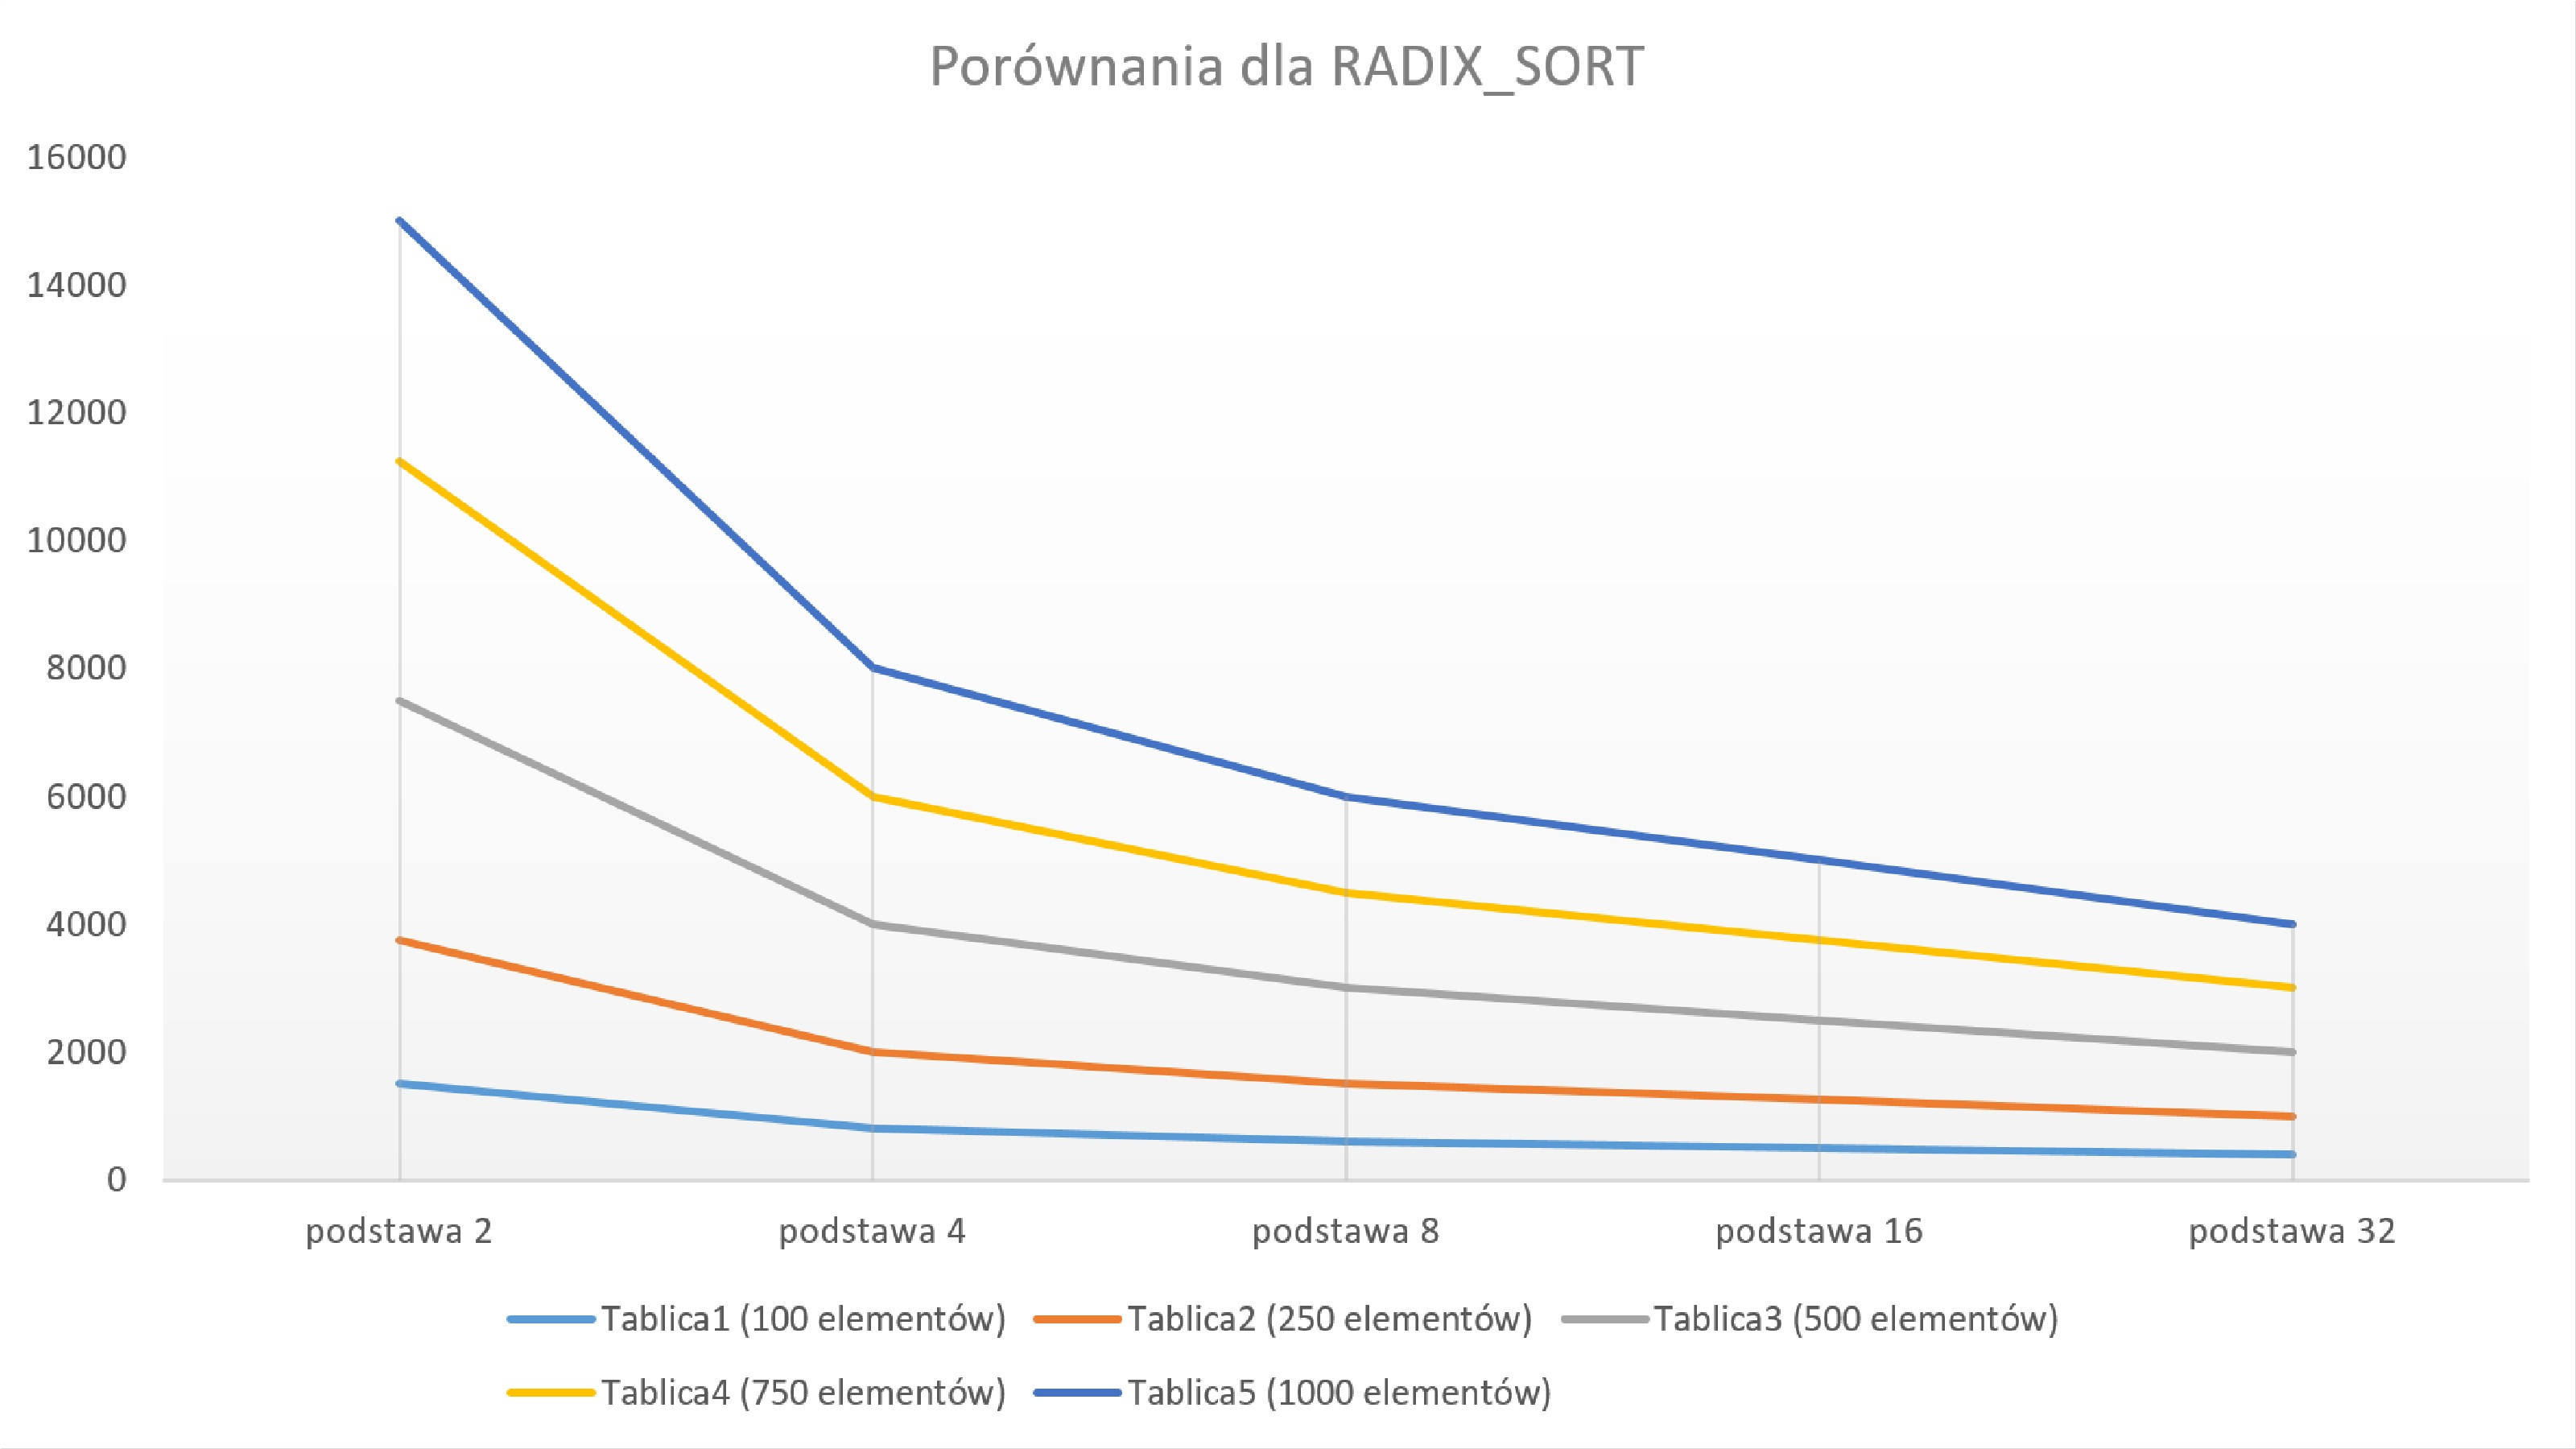
\includegraphics[width=1.0\textwidth]{POR2.jpg} 
		\end{figure}	
		\begin{table}[H]
			\centering
			\resizebox{\textwidth}{!}{
				\begin{tabular}{|c|c|c|c|c|c|}
					\hline
					\textbf{Przypisania} & \textbf{podstawa 2} & \textbf{podstawa 4} & \textbf{podstawa 8} & \textbf{podstawa 16} & \textbf{podstawa 32} \\ \hline
					\textbf{Tablica1 (100 elementów)}  & 1400  & 700  & 500  & 400  & 300   \\ \hline
					\textbf{Tablica2 (250 elementów)}  & 3500 & 1750 & 1250  & 1000  & 750   \\ \hline
					\textbf{Tablica3 (500 elementów)} & 7000 & 3500 & 2500  & 2000  & 1500  \\ \hline
					\textbf{Tablica4 (750 elementów)} & 10500 & 5250 & 3750  & 3000  & 2250  \\ \hline
					\textbf{Tablica5 (1000 elementów)} & 14000 & 7000 & 5000  & 4000  & 3000  \\ \hline
				\end{tabular}
			}
			\caption{Zestawienie ilości przypisań dla różnych podstaw w RADIX\_SORT.}
		\end{table}
		\begin{figure}[H]	
			\centering
			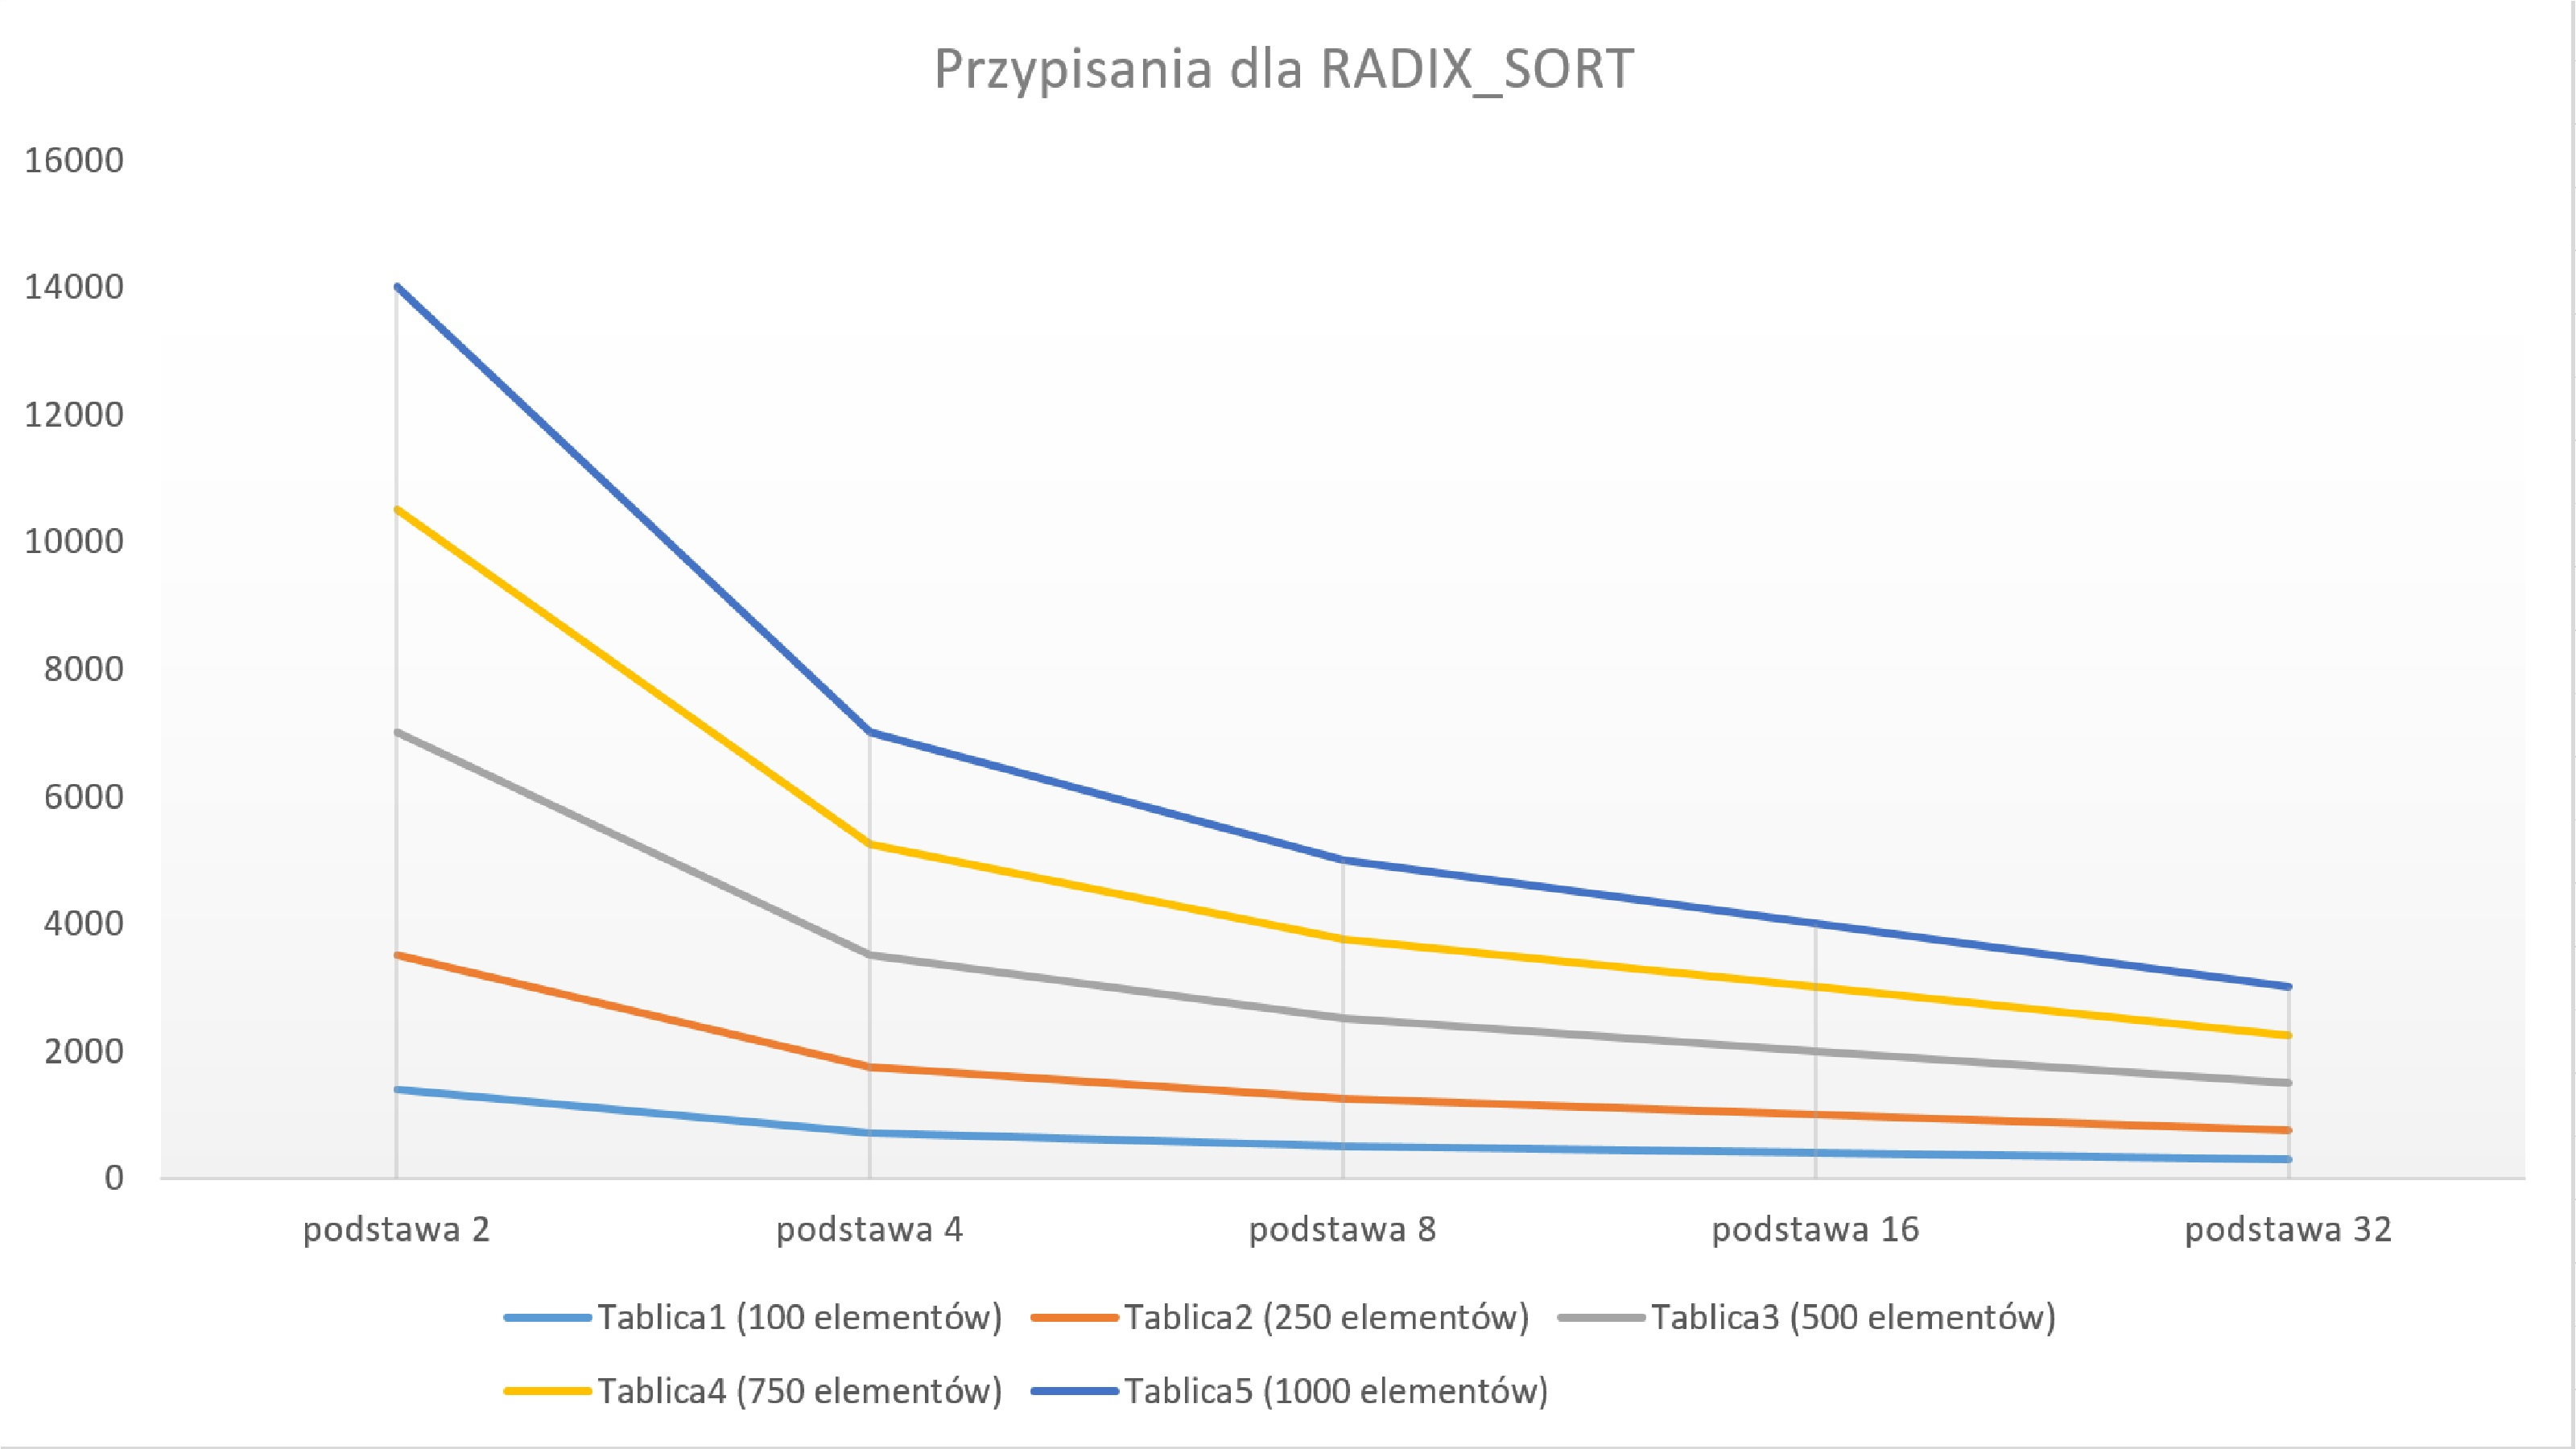
\includegraphics[width=1.0\textwidth]{PRZY2.jpg} 
		\end{figure}	
		\begin{table}[H]
			\centering
			\resizebox{\textwidth}{!}{
				\begin{tabular}{|c|c|c|c|c|c|}
					\hline
					\textbf{Porównania} & \textbf{podstawa 2} & \textbf{podstawa 4} & \textbf{podstawa 8} & \textbf{podstawa 16} & \textbf{podstawa 32} \\ \hline
					\textbf{Tablica1 (100 elementów)}  & 1598  & 898  & 698  & 598  & 498   \\ \hline
					\textbf{Tablica2 (250 elementów)}  & 3998 & 2248 & 1748  & 1498  & 1248   \\ \hline
					\textbf{Tablica3 (500 elementów)} & 7998 & 4498 & 3498  & 2998  & 2498  \\ \hline
					\textbf{Tablica4 (750 elementów)} & 11998 & 6748 & 5248  & 4498  & 3748  \\ \hline
					\textbf{Tablica5 (1000 elementów)} & 15998 & 8998 & 6998  & 5998  & 4998  \\ \hline
				\end{tabular}
			}
			\caption{Zestawienie ilości porównań dla różnych podstaw w RADIX\_SORT\_NEGATIVE.}
		\end{table}
		\begin{figure}[H]	
			\centering
			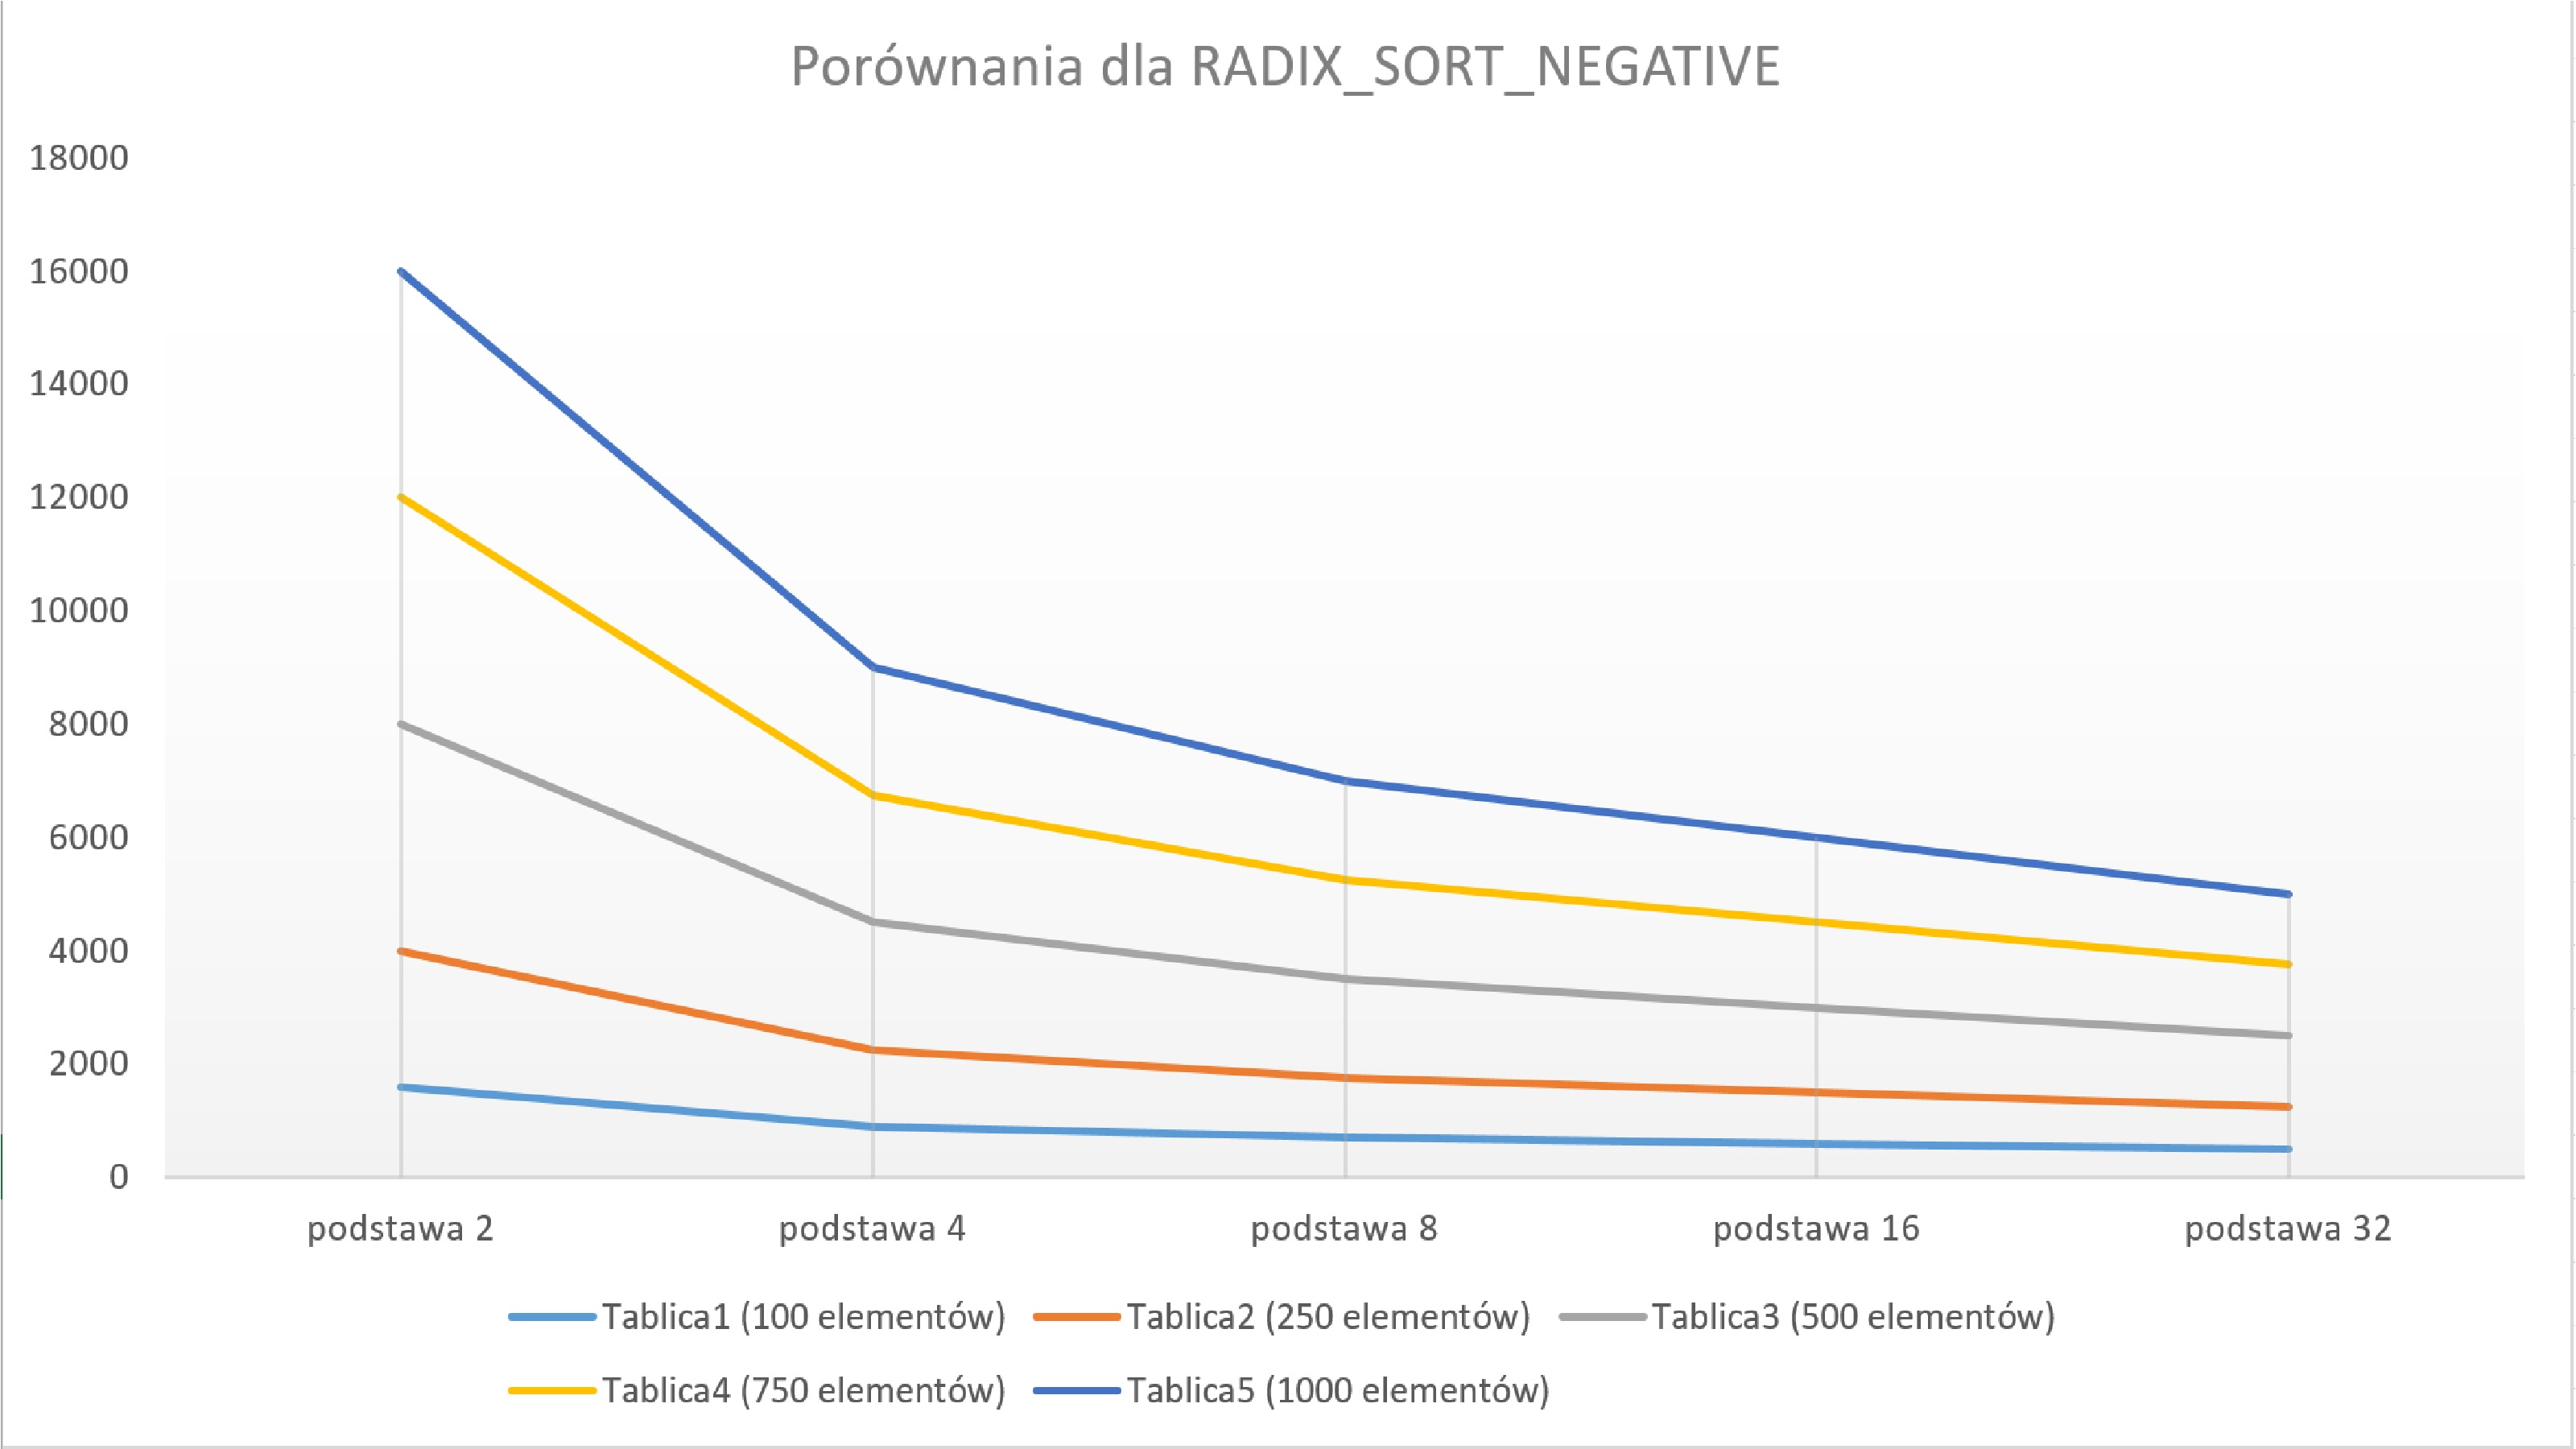
\includegraphics[width=1.0\textwidth]{POR3.jpg} 
		\end{figure}
		\begin{table}[H]
			\centering
			\resizebox{\textwidth}{!}{
				\begin{tabular}{|c|c|c|c|c|c|}
					\hline
					\textbf{Przypisania} & \textbf{podstawa 2} & \textbf{podstawa 4} & \textbf{podstawa 8} & \textbf{podstawa 16} & \textbf{podstawa 32} \\ \hline
					\textbf{Tablica1 (100 elementów)}  & 1600  & 900  & 700  & 600  & 500   \\ \hline
					\textbf{Tablica2 (250 elementów)}  & 4000 & 2250 & 1750  & 1500  & 1250   \\ \hline
					\textbf{Tablica3 (500 elementów)} & 8000 & 4500 & 3500  & 3000  & 2500  \\ \hline
					\textbf{Tablica4 (750 elementów)} & 12000 & 6750 & 5250  & 4500  & 3750  \\ \hline
					\textbf{Tablica5 (1000 elementów)} & 16000 & 9000 & 7000  & 6000  & 5000  \\ \hline
				\end{tabular}
			}
			\caption{Zestawienie ilości przypisań dla różnych podstaw w RADIX\_SORT\_NEGATIVE.}
		\end{table}
		\begin{figure}[H]	
			\centering
			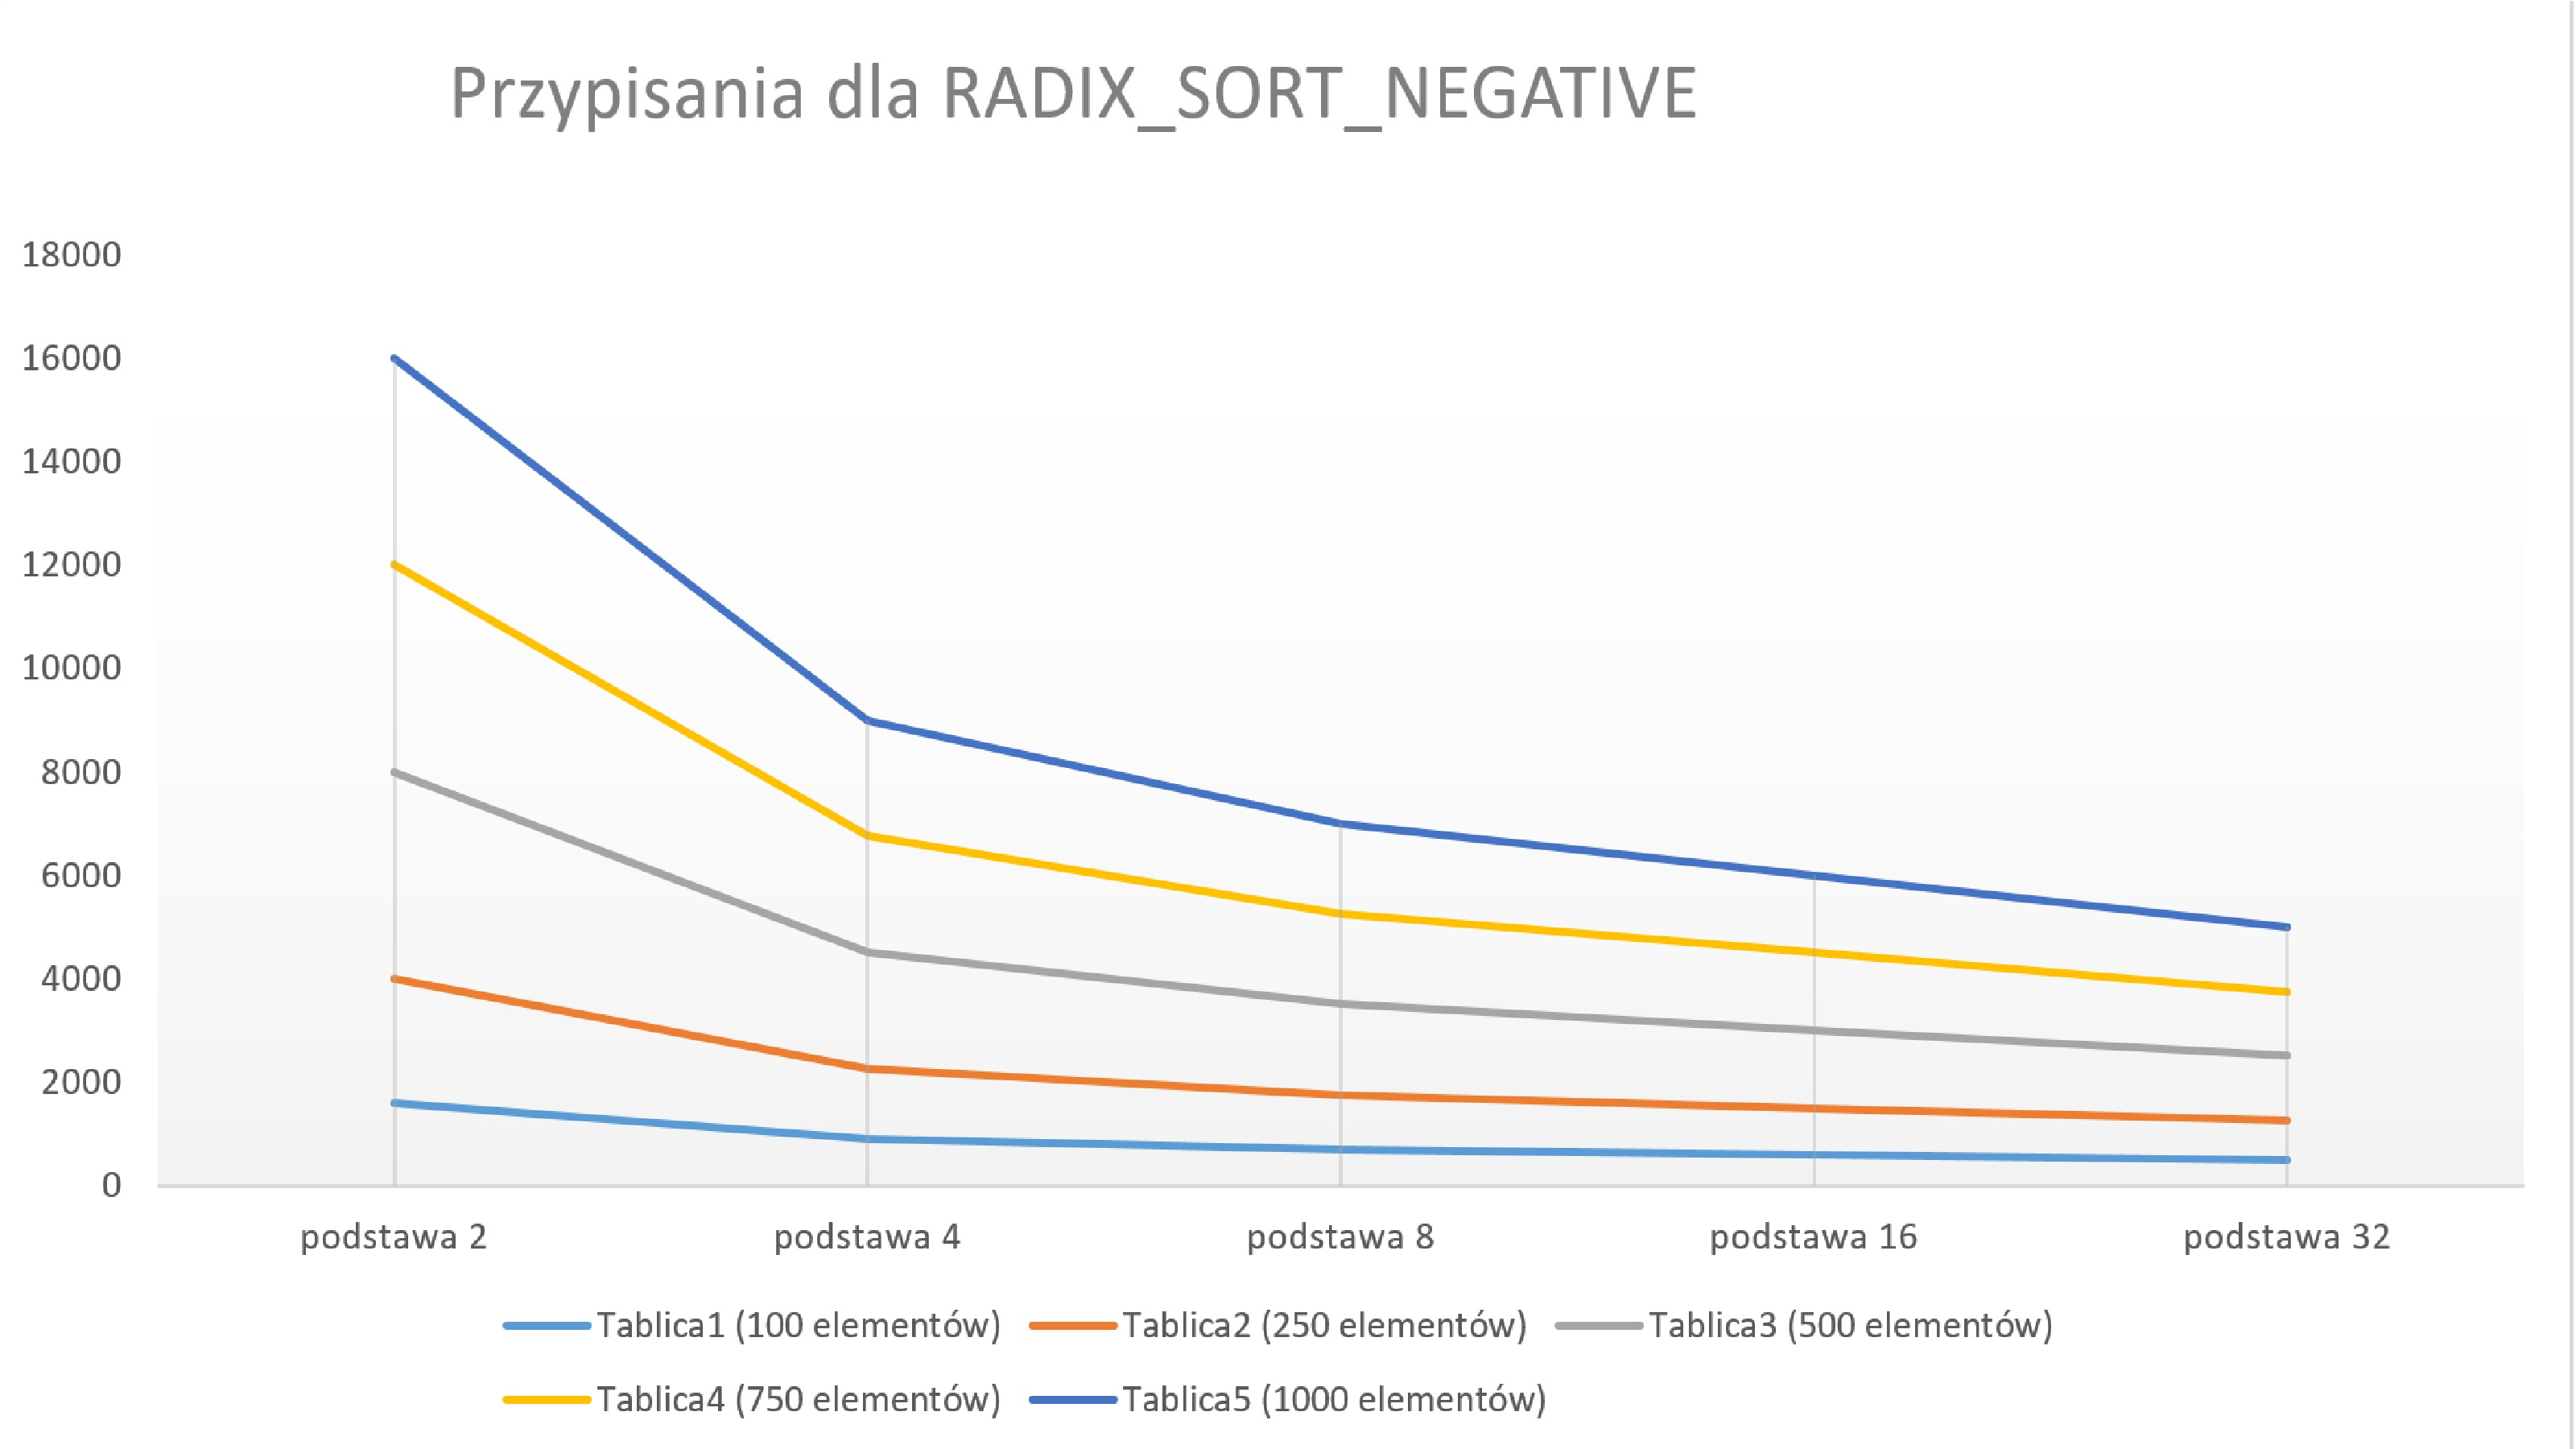
\includegraphics[width=1.0\textwidth]{PRZY3.jpg} 
		\end{figure}	
		Na podstawie przedstawionych tabel i wykresów, można zauważyć, że zarówno liczba porównań, jak i przypisań w algorytmie RADIX\_SORT oraz RADIX\_SORT\_NEGATIVE maleje wraz ze wzrostem wartości podstawy d. Dla każdej z wielkości tablic, wyniki wskazują, że przy większej podstawie, algorytm wykonuje mniej operacji, co oznacza poprawę efektywności.
		
		W przypadku podstawy d = 32, algorytm osiąga najniższe wartości zarówno dla porównań, jak i przypisań, co jest efektem zwiększenia zakresu przetwarzanych liczb w jednym kroku sortowania. Z kolei, przy najniższej podstawie d=2, liczba operacji jest najwyższa, ponieważ algorytm wymaga większej liczby iteracji oraz bardziej czasochłonnych operacji przy każdym z etapów sortowania.

		Zjawisko to jest widoczne szczególnie przy większych tablicach, gdzie różnice między wartościami porównań i przypisań przy różnych podstawach są bardziej wyraźne. Zwiększenie podstawy prowadzi do zmniejszenia liczby iteracji potrzebnych do przetworzenia wszystkich elementów, co obniża ogólny koszt obliczeniowy algorytmu. Różnice między wersjami RADIX\_SORT i RADIX\_SORT\_NEGATIVE są relatywnie niewielkie, ale ogólny trend malejącej liczby operacji jest zachowany w obu przypadkach.
		
	\section{Zadanie 6: Porównanie QUICK\_SORT i jego modyfikacji z BUCKET\_SORT}
	Testy przeprowadzono na pięciu tablicach o różnych rozmiarach (100, 250, 500, 750 i 1000 elementów), aby porównać wydajność algorytmów sortujących: quick\_sort, quick\_sort2, bucket\_sort1 oraz bucket\_sort2 pod względem liczby porównań i przypisań.
		\begin{table}[H]
			\centering
			\resizebox{\textwidth}{!}{
				\begin{tabular}{|c|c|c|c|c|}
					\hline
					\textbf{Porównania} & \textbf{quick\_sort} & \textbf{quick\_sort2} & \textbf{bucket\_sort1} & \textbf{bucket\_sort2} \\ \hline
					\textbf{Tablica1 (100 elementów)}  & 655  & 545  & 264  & 254   \\ \hline
					\textbf{Tablica2 (250 elementów)}  & 2015 & 2079 & 640  & 656   \\ \hline
					\textbf{Tablica3 (500 elementów)} & 4781 & 4591 & 1282  & 1329  \\ \hline
					\textbf{Tablica4 (750 elementów)} & 8610 & 8108 & 1937  & 1995  \\ \hline
					\textbf{Tablica5 (1000 elementów)} & 11302 & 12831 & 2552  & 2573  \\ \hline
				\end{tabular}
			}
			\caption{Zestawienie ilości porównań dla quick\_sort i bucket\_sort oraz ich modyfikacji.}
		\end{table}
		\begin{figure}[H]	
			\centering
			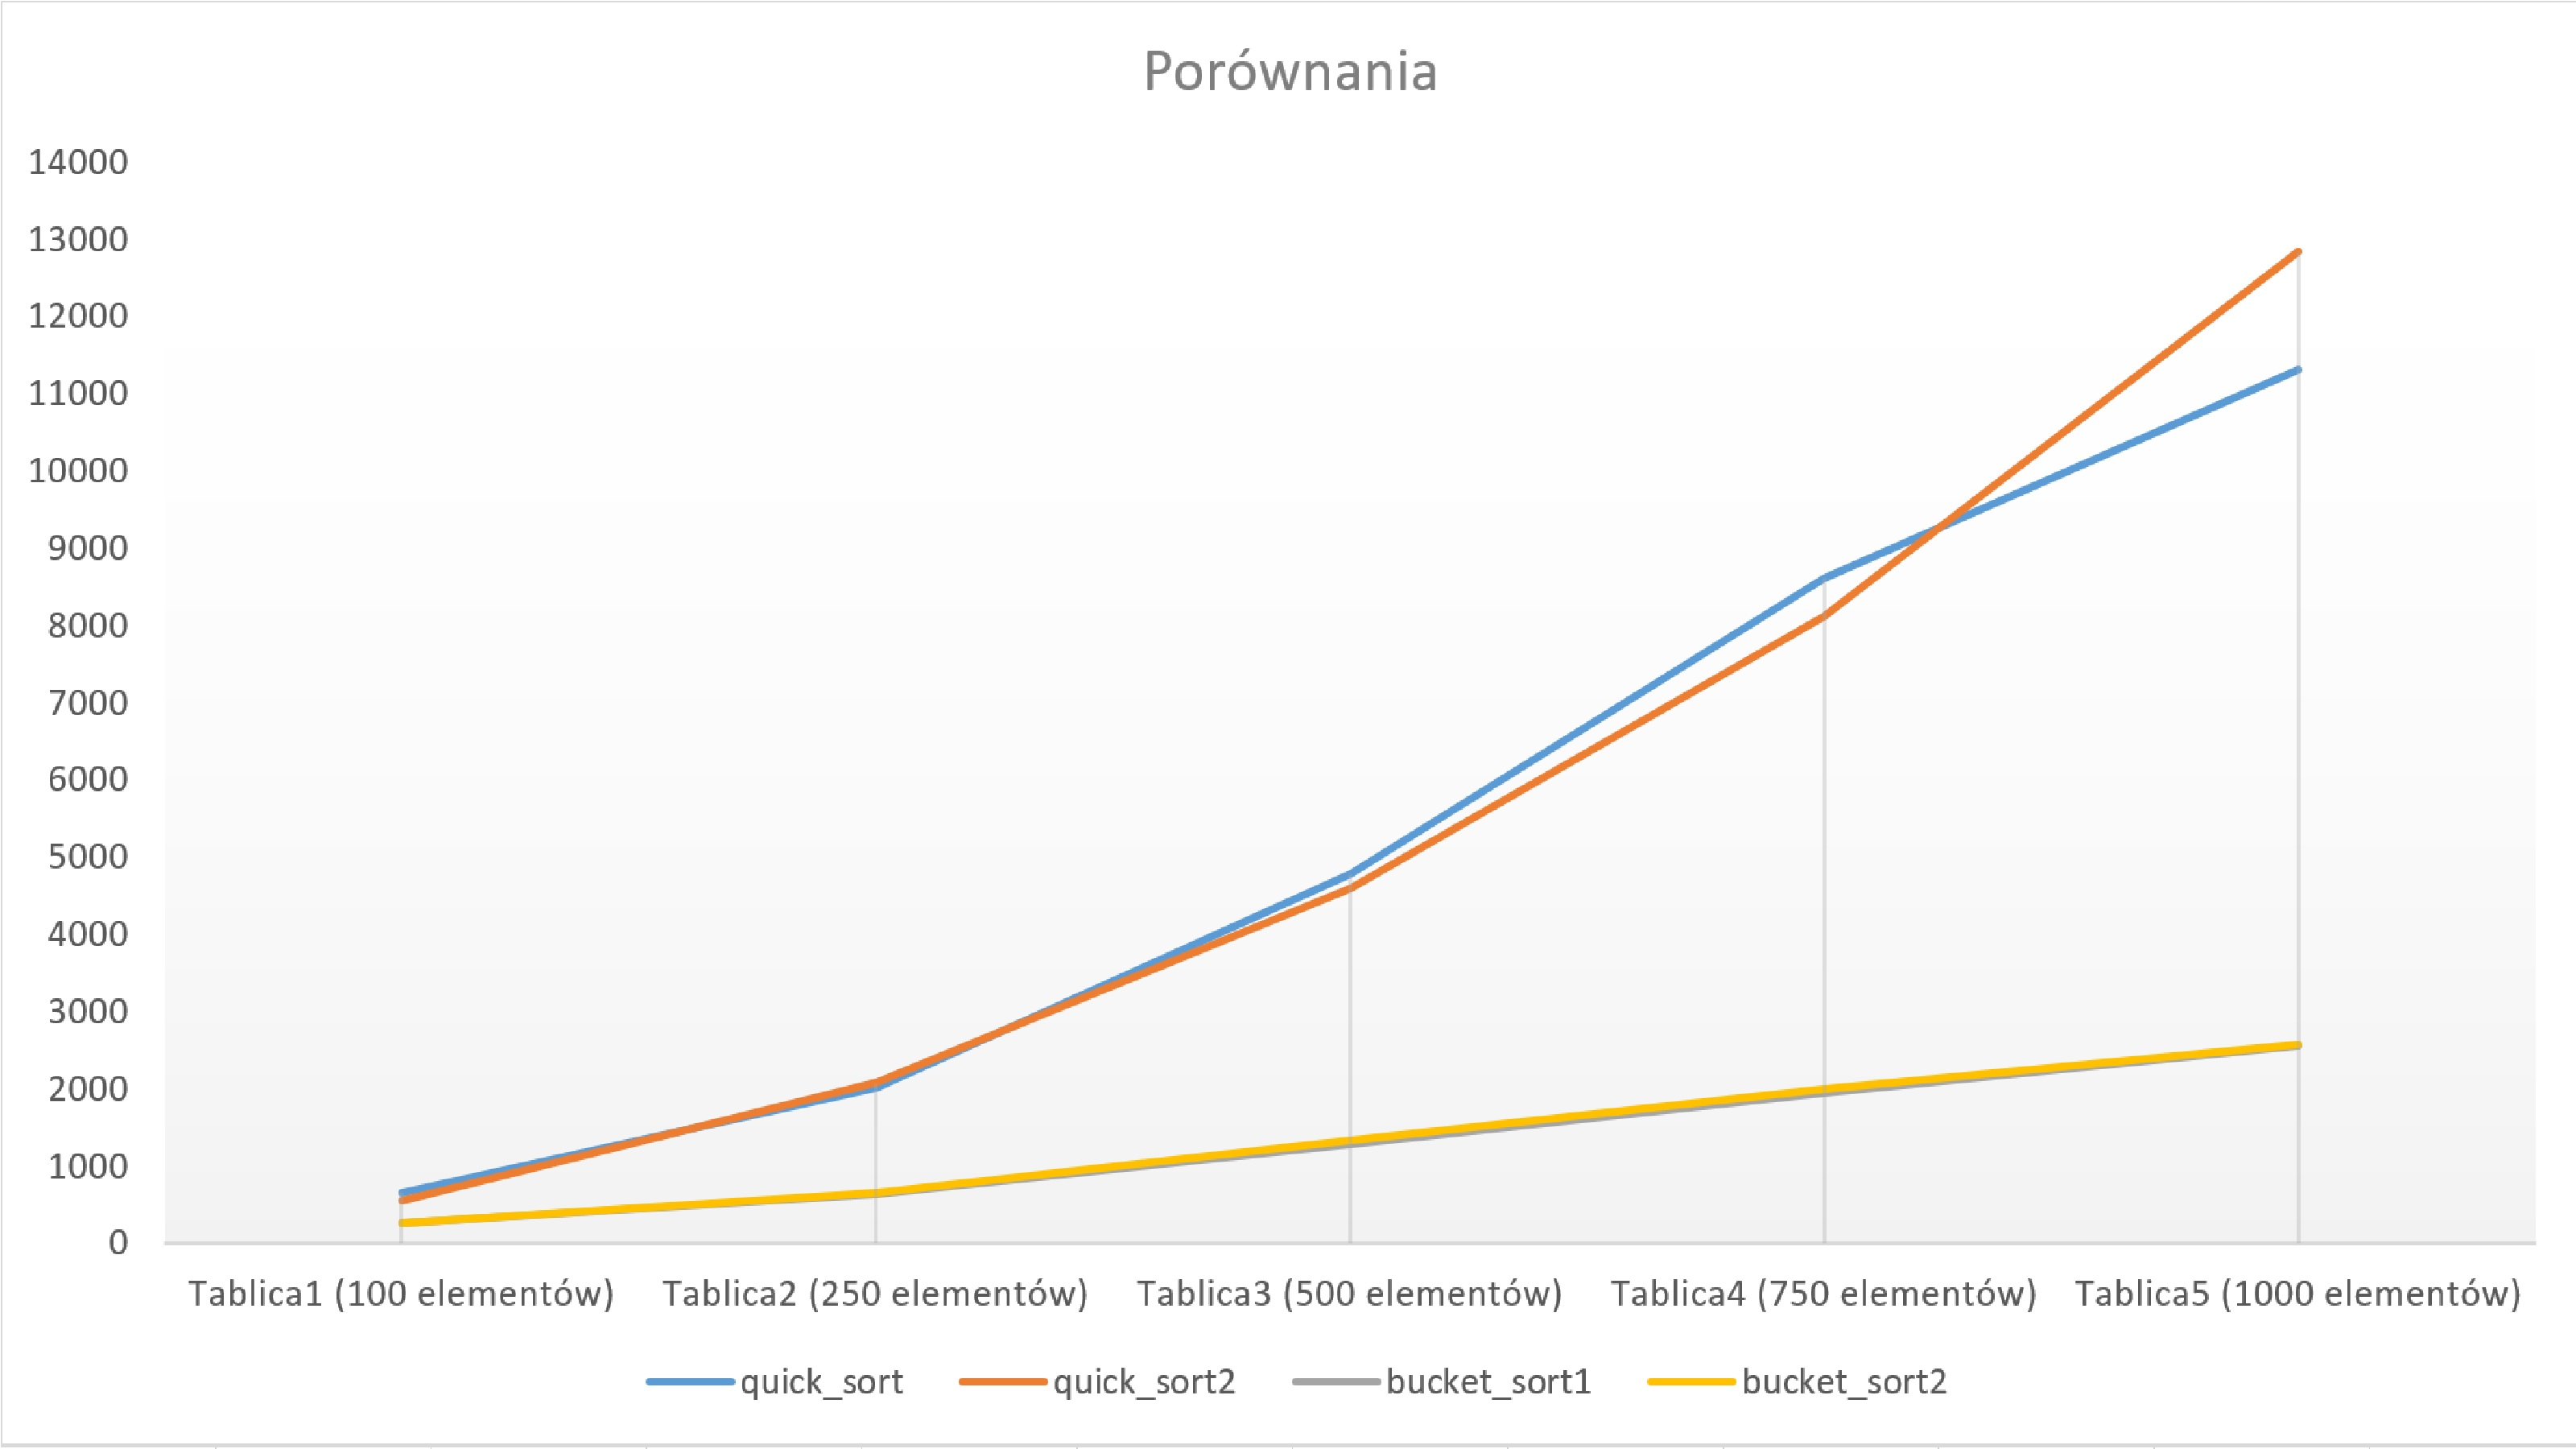
\includegraphics[width=1.0\textwidth]{POR1.jpg} 
		\end{figure}
		\begin{table}[H]
			\centering
			\resizebox{\textwidth}{!}{
				\begin{tabular}{|c|c|c|c|c|}
					\hline
					\textbf{Przypisania} & \textbf{quick\_sort} & \textbf{quick\_sort2} & \textbf{bucket\_sort1} & \textbf{bucket\_sort2} \\ \hline
					\textbf{Tablica1 (100 elementów)}  & 806  & 512  & 140  & 239   \\ \hline
					\textbf{Tablica2 (250 elementów)}  & 2708 & 1808 & 338  & 616   \\ \hline
					\textbf{Tablica3 (500 elementów)} & 6606 & 3966 & 671  & 1230  \\ \hline
					\textbf{Tablica4 (750 elementów)} & 8108 & 5862 & 1014 & 1856  \\ \hline
					\textbf{Tablica5 (1000 elementów)} & 12776 & 9578 & 1328 & 2351  \\ \hline
				\end{tabular}
			}
			\caption{Zestawienie ilości przypisań dla quick\_sort i bucket\_sort oraz ich modyfikacji.}
		\end{table}
		\begin{figure}[H]	
			\centering
			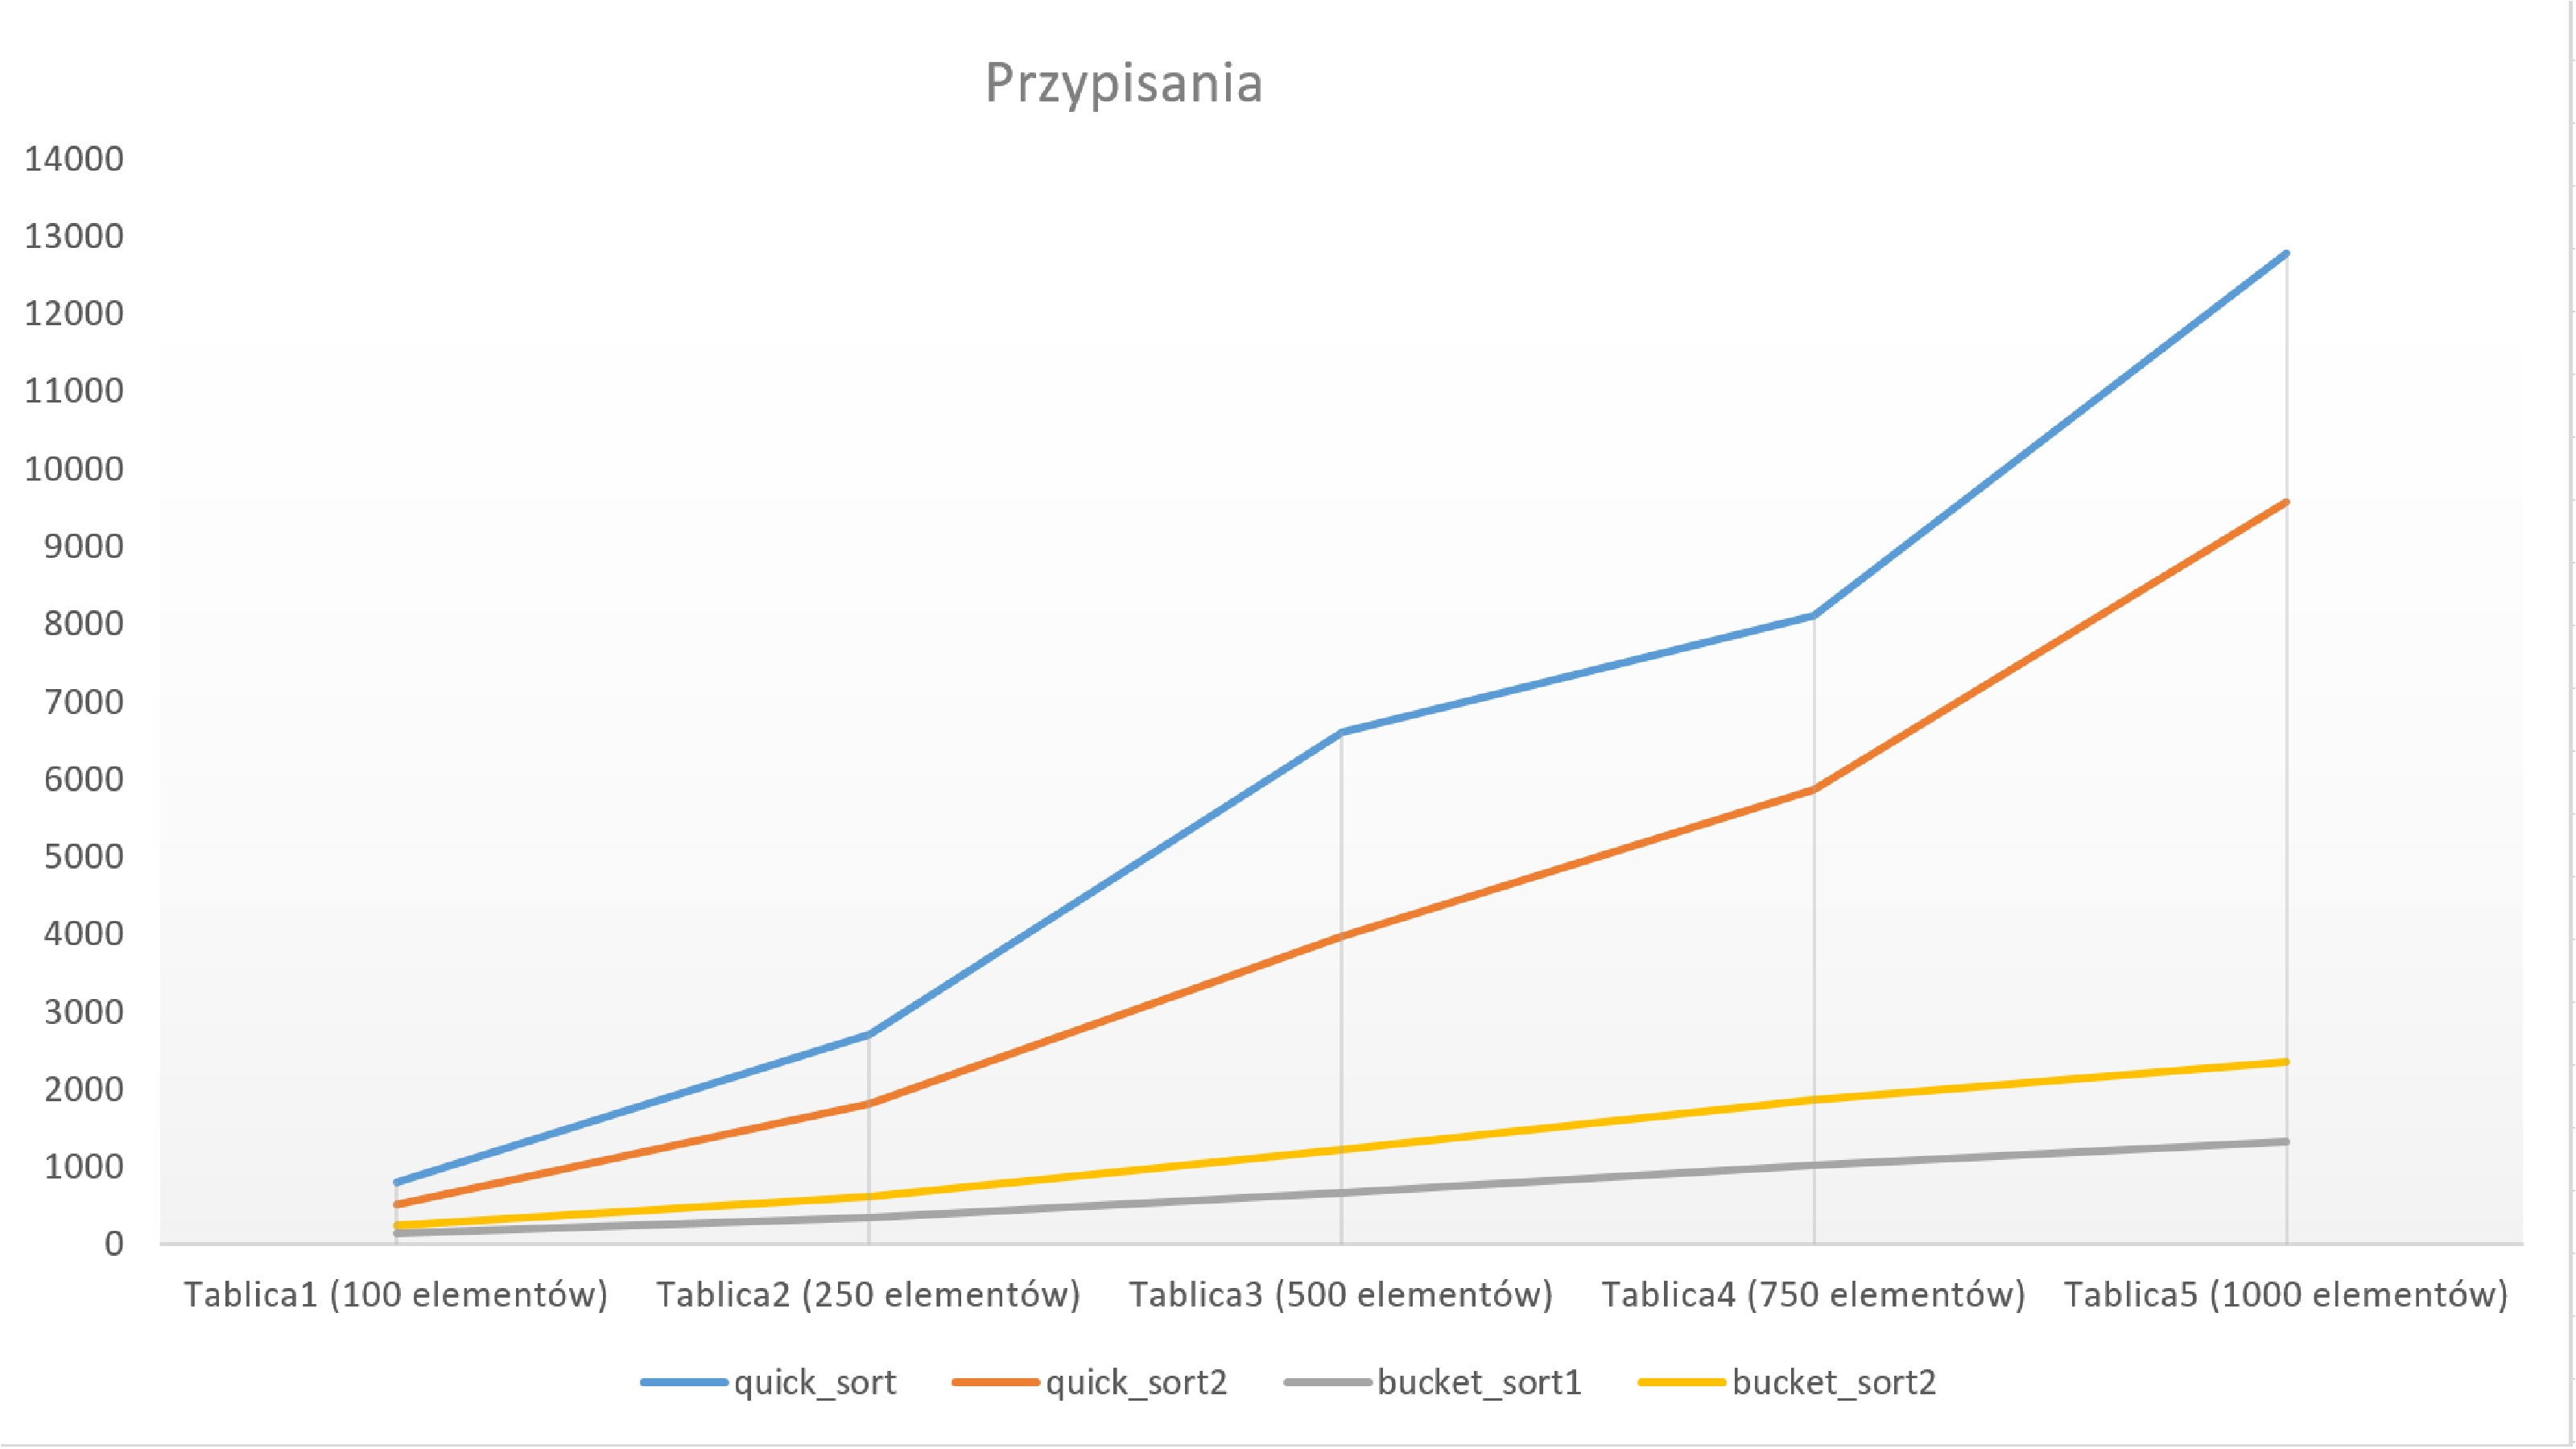
\includegraphics[width=1.0\textwidth]{PRZY1.jpg} 
		\end{figure}
		Na podstawie danych przedstawionych w tabelach i na wykresach, można zauważyć wyraźne różnice w wydajności algorytmów quick\_sort, quick\_sort2, bucket\_sort1 i bucket\_sort2 pod względem liczby porównań i przypisań.
		
		Zarówno liczba porównań, jak i przypisań rośnie wraz ze zwiększającym się rozmiarem tablicy, jednak różnice między algorytmami stają się bardziej widoczne przy większych rozmiarach danych. Bucket\_sort1 i bucket\_sort2 wykazują istotnie niższą liczbę porównań w porównaniu do quick\_sort i quick\_sort2, szczególnie dla większych tablic. To sugeruje, że algorytmy oparte na metodzie bucket sort są bardziej efektywne pod względem porównań, zwłaszcza przy większej liczbie elementów.
		
		Jeśli chodzi o liczbę przypisań, bucket\_sort również wypada korzystniej, wymagając mniej przypisań niż quick\_sort i jego modyfikacje, szczególnie w przypadku mniejszych tablic. Przy większych danych różnice w liczbie przypisań stają się wyraźniejsze, gdzie quick\_sort2 wymaga ich więcej niż algorytmy bucket\_sort.
		
	\section{Zadanie 7: Wnioski}
		Podsumowując wyniki przeprowadzonych testów, można stwierdzić, że im większa podstawa d w algorytmie Radix Sort, tym bardziej efektywnie algorytm przeprowadza sortowanie, co skutkuje zmniejszeniem liczby porównań i przypisań. Wzrost d poprawia skalowalność algorytmu, co czyni go bardziej wydajnym przy większych zbiorach danych.
		
		bucket\_sort i jego modyfikacje okazują się bardziej wydajne w zakresie liczby porównań i przypisań, szczególnie przy większych rozmiarach danych. Quick\_sort i quick\_sort2 osiągają zbliżone rezultaty przy mniejszych zbiorach danych, ale w miarę wzrostu rozmiaru tablicy, algorytmy oparte na metodzie bucket sort coraz wyraźniej przewyższają je pod względem efektywności.
\end{document}